

\tikzset{every picture/.style={line width=0.75pt}} %set default line width to 0.75pt        

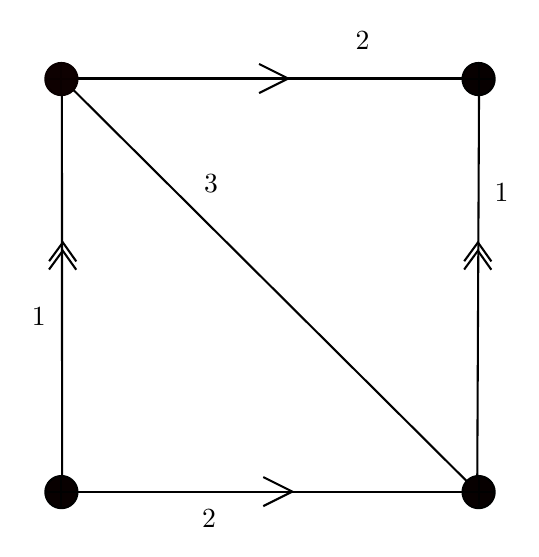
\begin{tikzpicture}[x=0.75pt,y=0.75pt,yscale=-1,xscale=1]
%uncomment if require: \path (0,487); %set diagram left start at 0, and has height of 487

%Straight Lines [id:da8215288959193072] 
\draw    (100,121) -- (100.08,320) ;
%Straight Lines [id:da8526418629967348] 
\draw    (301,120) -- (300.08,320) ;
%Straight Lines [id:da5367620041050422] 
\draw    (100.08,320) -- (300.08,320) ;
%Straight Lines [id:da4784595305292364] 
\draw    (100,121) -- (300,121) ;
\draw   (93.79,213.01) -- (100.41,203.96) -- (106.89,213.11)(93.82,209.01) -- (100.44,199.96) -- (106.92,209.11) ;
\draw   (293.79,213.01) -- (300.41,203.96) -- (306.89,213.11)(293.82,209.01) -- (300.44,199.96) -- (306.92,209.11) ;
\draw   (195,114) -- (209,121) -- (195,128) ;
\draw   (197,313) -- (211,320) -- (197,327) ;
%Straight Lines [id:da22151170816098675] 
\draw    (100,121) -- (300.08,320) ;
\draw  [color={rgb, 255:red, 10; green, 0; blue, 0 }  ,draw opacity=1 ][fill={rgb, 255:red, 14; green, 1; blue, 1 }  ,fill opacity=1 ] (92,121.25) .. controls (92,116.97) and (95.47,113.5) .. (99.75,113.5) .. controls (104.03,113.5) and (107.5,116.97) .. (107.5,121.25) .. controls (107.5,125.53) and (104.03,129) .. (99.75,129) .. controls (95.47,129) and (92,125.53) .. (92,121.25) -- cycle ; \draw  [color={rgb, 255:red, 10; green, 0; blue, 0 }  ,draw opacity=1 ] (92,121.25) -- (107.5,121.25) ; \draw  [color={rgb, 255:red, 10; green, 0; blue, 0 }  ,draw opacity=1 ] (99.75,113.5) -- (99.75,129) ;
\draw  [fill={rgb, 255:red, 7; green, 0; blue, 0 }  ,fill opacity=1 ] (293,121.25) .. controls (293,116.97) and (296.47,113.5) .. (300.75,113.5) .. controls (305.03,113.5) and (308.5,116.97) .. (308.5,121.25) .. controls (308.5,125.53) and (305.03,129) .. (300.75,129) .. controls (296.47,129) and (293,125.53) .. (293,121.25) -- cycle ; \draw   (293,121.25) -- (308.5,121.25) ; \draw   (300.75,113.5) -- (300.75,129) ;
\draw  [fill={rgb, 255:red, 8; green, 0; blue, 0 }  ,fill opacity=1 ] (92,320.25) .. controls (92,315.97) and (95.47,312.5) .. (99.75,312.5) .. controls (104.03,312.5) and (107.5,315.97) .. (107.5,320.25) .. controls (107.5,324.53) and (104.03,328) .. (99.75,328) .. controls (95.47,328) and (92,324.53) .. (92,320.25) -- cycle ; \draw   (92,320.25) -- (107.5,320.25) ; \draw   (99.75,312.5) -- (99.75,328) ;
\draw  [fill={rgb, 255:red, 7; green, 0; blue, 0 }  ,fill opacity=1 ] (293,320.25) .. controls (293,315.97) and (296.47,312.5) .. (300.75,312.5) .. controls (305.03,312.5) and (308.5,315.97) .. (308.5,320.25) .. controls (308.5,324.53) and (305.03,328) .. (300.75,328) .. controls (296.47,328) and (293,324.53) .. (293,320.25) -- cycle ; \draw   (293,320.25) -- (308.5,320.25) ; \draw   (300.75,312.5) -- (300.75,328) ;

% Text Node
\draw (84,230) node [anchor=north west][inner sep=0.75pt]   [align=left] {1};
% Text Node
\draw (307,170) node [anchor=north west][inner sep=0.75pt]   [align=left] {1};
% Text Node
\draw (166,327) node [anchor=north west][inner sep=0.75pt]   [align=left] {2};
% Text Node
\draw (240,97) node [anchor=north west][inner sep=0.75pt]   [align=left] {2};
% Text Node
\draw (167,166) node [anchor=north west][inner sep=0.75pt]   [align=left] {3};


\end{tikzpicture}
